\subsection{Obsidian} 
\label{sec:Obsidian} 
%\FloatBarrier

Obsidian is a programming language for expressing general purpose 
GPU kernels, compute kernels, in a high level and functional style.  
Obsidian is embedded in Haskell.
Specifically, Obsidian is a library of functions for generating 
and combining abstract syntax trees.
%That Obsidian is embedded in Haskell means that it is a library of 
%functions for generating and combining abstract syntax trees. 
By using features of Haskell such as overloading and higher-order-functions, 
the library/language border is blurred and we call the result an embedded 
language. From the abstract syntax trees generated while running an 
Obsidian program, NVIDIA CUDA code is generated. 


\subsubsection{A brief history of Obsidian} 
\label{sec:OBSHist}

In the Obsidian project we experiment with combinators and language 
features for GPU kernel implementation. We seek to strike a balance 
between low-level control and useful high-level abstractions. Over time, this 
has led to a number of different versions of Obsidian. In reference \cite{JSLIC}, 
two versions of Obsidian differing by having a {\em monadic} or a limited {\em arrow} 
like interface are described. We have settled on using the monadic style. 

One of the array representations that Obsidian uses, the Pull array, was present already 
in the earlier work but went under a different name. It was not until discovering 
a complementary array representation, that we call push arrays, that the traditional 
array was renamed to pull. 

The Obsidian implementation of pull arrays was influenced by Pan's representation 
of images as functions from coordinates to colour values \cite{PAN}. A pull array 
is a function from index to value and an associated length.  

Push arrays were added to Obsidian first in reference \cite{Obsidian-Expressive}. A push array
specifies where elements are to end up in a result array, rather than where 
they come from (as in a pull array). In essence, a push array is a
computation which writes an array to memory, but is parameterised on
the {\em write function} which writes a single element into memory.
The push array function can then 
use the write function zero, one, or several times. 

Push arrays were added to Obsidian with the purpose of solving some performance 
issues that we had been struggling with for a long time. These problems were 
mainly concerned with concatenating or combining arrays in an efficient way.
Push arrays have also been adopted by others and are used in the implementation 
of filters in reference~\cite{FPCDSL} and in the new Nikola\footnote{github.com/mainland/nikola/blob/master/src/Data/Array/Nikola/Repr/Push.hs}.

Both push and pull arrays are virtual, in the sense that they do not directly 
correspond to any data in a region of memory. This virtual nature of the array 
representations gives us fusion of operations for free. The programmer has 
to explicitly force an array (using a {\tt force} function) to actually compute 
the values and store them in memory and to prevent operations from fusing. 

In the version of Obsidian used in this paper\footnote{github.com/svenssonjoel/Obsidian/branches/February2013}, new features were added.  We 
introduce two new variants of push and pull arrays called {\tt GlobPush} and 
{\tt GlobPull}. This introduces a distinction between local arrays, short 
enough to be computed by a block of the GPU, and global arrays that represent 
computations spread over blocks of the GPU. This is an important step when 
it comes to Obsidian's capabilities; we can now express in what order a kernel
fetches elements from global memory. 
Earlier versions of Obsidian were limited to straight-line block indexing. A kernel 
generated by older Obsidian accessed blocks of elements in a fixed way (thread block 
i accessed elements using {\tt (i * blocksize) + f tid}, where {\tt f} can permute 
indices within a block but there is no similar way to permute the actual blocks). 

In order to implement histograms we also need to add  atomic operations to the language. The addition of atomic operations here is 
done in a rather ad hoc way and pushes us to program in a very low-level and 
imperative style. We strive to incorporate much of CUDA's low-level functionality 
into Obsidian and adding atomic operations is an attempt in that 
direction.  

The version of Obsidian used in this paper also introduces a new monadic representation 
of GPU programs. We call the monad {\tt Program}. The {\tt Program} type has a 
parameter that represents at what level in the GPU hierarchy it executes. There 
are sequential {\em Thread} programs and parallel {\em Block} and {\em Grid} programs. Type synonyms 
are available, {\tt TProgram}, {\tt BProgram} and {\tt GProgram}.   

Many of the new features we mention above have been further refined and 
are present in versions of Obsidian following the one we use in this paper. For 
example, in the master branch of Obsidian\footnote{github.com/svenssonjoel/Obsidian} we build on the ideas in this paper. 
There, global and local arrays are represented by the same data type. That 
work also goes further by implementing hierarchy generic functions that are 
applicable at different levels of the Thread, Block and Grid hierarchy. 
We are also experimenting with the addition of mutable arrays in order to 
better integrate the atomic operations\footnote{github.com/svenssonjoel/Obsidian/tree/mutable}. 




%% Obsidian raises the level of abstraction for GPU programming but wants 
%% to keep low level control. To facilitate this, Obsidian supplies different 
%% kinds of arrays. There are {\tt Push} and {\tt Pull} arrays for local 
%% computations and in the current version of 
%% Obsidian\footnote{github.com/SvenssonJoel/Obsidian} we add global arrays 
%% of types {\tt GlobPush} and {\tt GlobPull} to the language.

%% Both push and pull arrays are in some sense virtual. They do not necessarily 
%% represent data that exists in memory. Instead, the push and pull arrays 
%% represent ways to compute an array. Concretely, a pull array is function from 
%% index to element. A push array is a function that when given a write-function 
%% (a function that takes an index and an element to a program 
%% that represents the writing of that element into an array) gives 
%% a program that represents writing a number of elements. In 
%% Obsidian, there are three kinds of programs, represented by a {\tt Program} data 
%% type. TPrograms, BPrograms and GPrograms represent what a thread, block of 
%% threads and a grid of blocks can do. Thread programs are the result type in 
%% the so-called write-functions. BPrograms operate on local arrays and 
%% grid programs operate on global arrays. 
%% Since push and pull arrays are virtual operations upon them are fused 
%% automatically. The standard example is map-fusion {\tt (map a . map b = map (a . b))}. 
%% The programmer decides when, and if, intermediate values are computed and 
%% stored in memory by using a {\tt force} function.
%% %In order to ensure that an intermediate value is computed there is a {\tt force}
%% %function. 
%% The {\tt force} function takes a push or pull array and gives 
%% a block program resulting in a pull array. The block program writes the data 
%% contained in the array into shared memory and the return array symbolises 
%% reading from that memory. 
  
%% %Hence, when working with local push and 
%% %pull arrays the associated programs are thread and block programs and when 
%% %working with global arrays the grid programs also come into play.  

%% The push and pull arrays have different strengths. Pull arrays 
%% make it easy to implement functions such as {\tt map} and {\tt zipWith}. 
%% % and 
%% %also give map-fusion for free. A pull array is also easy to parallelise;  
%% %thread $i$ is in charge of computing element $i$.  
%% %The push arrays provide ways to compute arrays in a way so that thread $i$ 
%% %computes other elements than $i$. Actually, any thread be in charge of the 
%% %computation of any element of the result. 
%% Push arrays allow thread $i$ to compute array elements at indices other 
%% than $i$; this enables efficient array concatenation as well 
%% as the data scattering operations used later. For more information about 
%% push arrays, see reference \cite{PUSH}. 

%Both push and pull arrays are easy to parallelise. 
 
%In the current version of Obsidian\footnote{github.com/SvenssonJoel/Obsidian} 
%we are exploring ways to increase the scope of what kinds of compute kernels 
%we can describe and obtain efficient code for. One aspect of this exploration 
%is the addition of a new kind of array representation that we call 
%{\em push} arrays \cite{PUSH}. Previous versions of Obsidian 
%(described in \cite{JSLIC}) represented arrays as functions 
%from indices to values,we call these {\em pull} arrays. Another addition 
%is global arrays. Earlier versions of Obsidian has been focused on 
%expressing the kind of computations that takes place locally, in a block.  
 
%The pull representation of arrays make it easy to describe 
%functions that take arrays apart and gives fusion of operations (for 
%example map-fusion) for free. However, Combining arrays, such as the 
%array concatenate operation, is not efficient using this array 
%representation. We have had problems in generating good CUDA code 
%for such functions. For example concatenation of pull arrays 
%leads to conditionals in the generated code of a kind that can have 
%negative performance impact on the GPUs we are targeting. 
%The implementation of the algorithm described in this paper 
%uses both the pull and the push arrays offered by Obsidian. 

%The GPUs targeted by Obsidian has an hierarchical structure 
%in more senses than just its memory system. Threads are only 
%allowed to communicate using local shared memory in small groups 
%(thread blocks). 
%To match the hierarchal architecture of GPUs, Obsidian has local arrays 
%of type {\tt Pull a} and {\tt Push a}. These local arrays are used in the 
%implementation of programs that can be run by a block, in Obsidian these 
%programs are represented by a data type called {\tt BProgram}. There 
%are also global arrays types {\tt GlobPull a} and {\tt GlobPush a} that 
%are used in the implementation of programs executed by more than one MP, 
%these programs are represented by a {\tt GProgram} data type.   
%and global arrays of 
%types {\tt GlobPull a} and {\tt GlobPush a}.
%Global arrays are used when simple permutations of a large input array is 
%needed. Here it is important to that no communication needing 
%synchronisations occurs. Global arrays are also used as the inputs 
%and outputs of a top level Obsidian program (a program you want to generate runnable CUDA code from). In the cases where threads need to cooperate 
%on solving a task the local arrays should be used. 
\subsubsection{Obsidian programming example} 
\label{sec:sklansky}
\FloatBarrier

In the different variants of counting sort that are developed in this
paper, the prefix sum operation is the same. It is therefore natural
to use as an introductory example of how Obsidian programs are
written.

%We want to be able to sort large arrays and to do this we need an 
%implementation of prefix sum that is larger (on more elements) than what 
%fits in a block. 
We need to operate on arrays that are too long to fit in a single block.
%This large prefix sum is implemented as shown in
The resulting prefix sum is implemented as shown in reference 
\cite{ScanCUDA}, see figure \ref{fig:prefixsum}. There are three steps 
involved. First local prefix sums are computed; the rightmost elements elements are also stored in a separate, auxiliary, array. Following this, 
the prefix sum of the auxiliary array is  computed. The prefix sums used 
in phase A and B of the 
figure can both be generated from the same Obsidian program. Finally the 
local prefix sums and the result of the auxiliary prefix sum are combined, 
forming a large prefix sum over the entire array. 

\begin{figure}
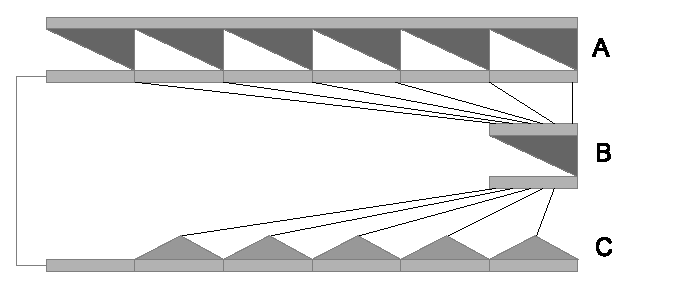
\includegraphics[width=\linewidth]{./csort/prefixsum}
\caption{Illustration of how to combine many local prefix sum computations 
 into a large one. The algorithm has three steps: A compute local prefix sums, 
 B recursively compute prefix sums on the maximums of the local prefix sum 
 calculations, C distribute summed maximums over the local results.}
\label{fig:prefixsum}
\end{figure}

\begin{figure} 
\begin{center}
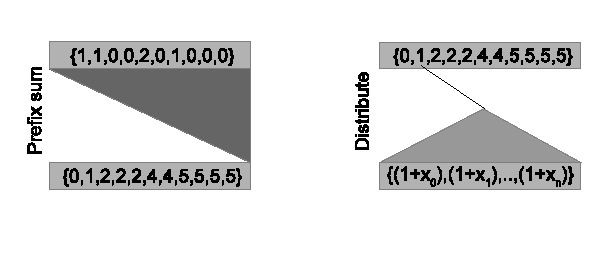
\includegraphics[width=\linewidth]{./csort/prefixzoom}
\caption{Close-up on the prefix sum and distribute operations used in Figure \ref{fig:prefixsum}.} 
%Zooms in on the shapes used in figure \ref{fig:prefixsum}. The left 
%shape symbolises a prefix sum and the right shows the distribute operation}
\label{fig:prefixzoom}
\end{center}
\end{figure}

The figure also shows what kernels we need to produce. First, something that 
performs a number of local prefix sums in parallel over the full length 
of an array is needed. The prefix sum algorithm that we implement here is 
based on divide and conquer and originates from Sklansky \cite{Sklansky}. 
% A kernel that performs the distribution (part C in the figure) is also needed. 

The code below can be thought of as a program generator. Given an integer, $n$,
it gives a prefix computation for $2^n$ elements. Here we go directly to 
generating the prefix sums operations (with the operator + hard coded) rather 
than a higher order function that can be used to more generically.

\begin{small}
\begin{Verbatim}[samepage=true]
sklansky :: Int 
            -> Pull EWord32 
            -> BProgram (Pull EWord32)
sklansky 0 arr = return arr
sklansky n arr = do 
    let arr1 = binSplit (n-1) fan arr
    arr2 <- force arr1
    sklansky (n-1) arr2
\end{Verbatim}
\end{small} 

%\begin{small}
%\begin{verbatim} 
%sklansky :: Scalar a => Int -> (Exp a -> Exp a -> Exp a)
%            -> Pull (Exp a) -> BProgram (Pull (Exp a))
%sklansky 0 op arr = return arr
%sklansky n op arr = do 
%    let arr1 = binSplit (n-1) (fan op) arr
%    arr2 <- force arr1
%    sklansky (n-1) op arr2
%\end{verbatim}
%\end{small} 

The {\tt sklansky} code above is short but still contains much that needs 
explanation. First, the type specifies that the function takes a normal 
Haskell Int and an input array ({\tt Pull EWord32}). The result is a {\tt BProgram} that 
produces a result array. 
%The code above could be thought of as a program 
%generator for a supplied number,$n$, and operation (for example (+)); it gives 
%you a program that performs all prefix sums operation on an array. 
The function {\tt binSplit} is in the Obsidian library and is used 
to implement divide and conquer algorithms. This function splits an array 
recursively a given number of times and then applies some computation on all 
parts. In this case the {\tt fan} operation implemented below is used. 

%To be able to implement prefix sum on the GPU we need to split the work 
%up into different phases. While computing a prefix sum in parallel , values 
%needs to be communicated between threads. This indicates that a kernel that 
%utilises local shared memory is a good idea. In CUDA the threads that can 
%communicate via shared memory all belong to the same block (group of threads). 
%These blocks can contain up to 1024 threads but often much fewer to 
%conserve resources and allow more blocks to run in parallel. In this example 
%a 256 threads (and elements) kernel is created. In the 
%benchmarks (section \ref{sec:Benchmarks}) prefix sum kernels of many 
%different sizes are used but all of these can be generated from the same 
%Obsidian description. In order to be able to implement a large prefix sum 
%the local kernel is also designed to output its maximal element to 
%a separate array. This separate array can be used to compute values to adjust 
%the local sums by. This follows the schema developed in \cite{LargeScan}.

%The local prefix sum is executed in parallel over the large array. 
%The large array is thus some multiple of the number of elements that the 
%local kernel can process. These sub results (both local scans and recursively 
%scaned block maximi) are then combined using another kernel called 
%{\tt distribute}. 

%\begin{verbatim} 
%sklansky :: Scalar a => Int -> (Exp a -> Exp a -> Exp a)
%            -> Pull (Exp a) -> BProgram (Pull (Exp a))
%sklansky 0 op arr = return arr
%sklansky n op arr = do 
%    let arr1 = twoK (n-1) (fan op) arr
%    arr2 <- force arr1
%    sklansky (n-1) op arr2
%\end{verbatim}

\begin{small}
\begin{Verbatim}[samepage=true]
fan arr =  a1 `conc`  fmap (+ (last a1)) a2 
    where 
      (a1,a2) = halve arr
\end{Verbatim} 
\end{small}
%\begin{small}
%\begin{verbatim} 
%fan op arr =  a1 `conc`  fmap (op c) a2 
%    where 
%      (a1,a2) = halve arr
%      c = a1 ! (fromIntegral (len a1 - 1))
%\end{verbatim} 
%\end{small}


The {\tt fan} operation splits an array down the middle and then adds 
the element at the highest index of the first half to all elements of 
the second. Then the two parts are concatenated back together. 
%The {\tt sklansky} function uses the {\tt force} function that ensures 
%that the array is computed and the elements stored in memory. This can be 
%used to introduce parallelism but also, by leaving it out, to ensure fusion 
%of computations. 

In order to obtain both the local prefix sum results and the maximum 
element of the block, a small wrapper function is created. 

\begin{small}
\begin{Verbatim}[samepage=true]
sklanskyMax :: Int 
               -> Pull EWord32 
               -> BProgram (Pull EWord32, 
                            Pull EWord32)
sklanskyMax n arr = do
  res <- sklansky n arr
  return (res,singleton (last res))
\end{Verbatim}
\end{small} 
%\begin{small}
%\begin{verbatim}
%sklanskyMax :: Scalar a => Int -> (Exp a -> Exp a -> Exp a)
%     -> Pull (Exp a) -> BProgram (Pull (Exp a), Pull (Exp a))
%sklanskyMax n op arr = do
%  res <- sklansky n op arr
%  return (res,singleton (last res))
%\end{verbatim}
%\end{small} 

All this wrapper does is compute the prefix sum followed by returning the  
result and a singleton array containing the maximum, {\tt last}, element. 

%This function is currently the 
%target of much experimentation with regards to how exactly it should 
%be implemented and what exact type it should have.
This local prefix sum is run on sub-parts of the global array. The function
{\tt mapDist} splits up the array, runs a local computation on each part using
the MPs of the GPU; when it finishes, the result of that computation is an array
that remains distributed across the local memories of the GPU MPs. 

\begin{small}
\begin{Verbatim}[samepage=true]
sklanskyG :: Int 
             -> GlobPull EWord32
             -> GProgram (GlobPush EWord32, 
                          GlobPush EWord32)
sklanskyG logbsize input =
  toGProgram (mapDist (sklanskyMax logbsize) 
                      (2^logbsize) 
                      input)
\end{Verbatim}  
\end{small}
%\begin{small}
%\begin{verbatim} 
%sklanskyG :: (Num (Exp a), Scalar a)
%             => Int
%             -> GlobPull (Exp a)
%             -> GProgram (GlobPush  (Exp a), GlobPush (Exp a))
%sklanskyG logbsize input = toGProgram $
%    mapDist (sklanskyMax logbsize (+)) (2^logbsize) input
%\end{verbatim}  
%\end{small}


In the {\tt sklanskyG} function the local prefix combinator implemented 
so far is turned into a global prefix sum computation. 
The {\tt toGProgram} function takes a function from blockId to 
a {\tt BProgram} and gives back a {\tt GProgram}, that is a program running 
on the full GPU (across many MPs). 

The CUDA code generated from {\tt sklanskyG} is shown in figure
\ref{fig:genSklansky}. Writing that type of CUDA code by hand is both
tedious and error prone. The Obsidian code is both shorter, more
compositional and easier to read.

One kernel remains to be implemented, {\tt distribute}.

\begin{small}
\begin{Verbatim}[samepage=true]
distribute :: EWord32 
              -> GlobPull EWord32
              -> GlobPull EWord32 
              -> GlobPull EWord32
distribute bs maxs inputs = zipWithG (+) maxs' inputs 
  where 
    maxs' = repeat bs maxs
    repeat n = ixMap (\ix -> ix `div` n)
\end{Verbatim} 
\end{small}
%\begin{small}
%\begin{verbatim} 
%distribute :: Num a => Exp Word32 -> GlobPull a 
%              -> GlobPull a -> GlobPull a
%distribute bs maxs inputs = zipWithG (+) maxs' inputs 
%  where 
%    maxs' = repeat bs maxs
%    repeat n gp = ixMap (\ix -> ix `div` n) gp 
%\end{verbatim} 
%\end{small}
%repeat n (GlobPull ixf) = GlobPull $ \ix -> ixf (ix `div` n) 

The {\tt distribute} kernel takes three inputs, a number, $n$,  and two global pull 
arrays. The elements of the first array are repeated $n$ times and then 
the result is element wise added to the second input array. The code generated 
from this kernel is shown in figure \ref{fig:genDistrib}. The 
{\tt distribute} kernel is used in the implementation of a large prefix sum 
(over more elements then what can fit in shared memory) from local prefix sum 
computations. This is indicated in figure~\ref{fig:prefixsum}.

\begin{figure} 
\newcommand{\myfontsize}{\fontsize{7}{9}\selectfont}
{\myfontsize
\begin{verbatim} 
__global__ void sklansky(uint32_t *input0,
                         uint32_t *output0,
                         uint32_t *output1){
  extern __shared__ unsigned char sbase[];
  ((uint32_t *)sbase)[tid] = 
    (((tid&0x1)<0x1) 
      ? input0[((bid*32)+((tid&0xFFFFFFFE)|(tid&0x1)))] 
      : (input0[((bid*32)+((tid&0xFFFFFFFE)|0x0))]+
         input0[((bid*32)+((tid&0xFFFFFFFE)|(tid&0x1)))]));
  __syncthreads();
  ((uint32_t *)(sbase + 128))[tid] = 
    (((tid&0x3)<0x2) 
      ? ((uint32_t *)sbase)[((tid&0xFFFFFFFC)|(tid&0x3))] 
      : (((uint32_t *)sbase)[((tid&0xFFFFFFFC)|0x1)]+
         ((uint32_t *)sbase)[((tid&0xFFFFFFFC)|(tid&0x3))]));
  __syncthreads();
  ((uint32_t *)sbase)[tid] = 
    (((tid&0x7)<0x4) 
      ? ((uint32_t *)(sbase+128))[((tid&0xFFFFFFF8)|(tid&0x7))] 
      : (((uint32_t *)(sbase+128))[((tid&0xFFFFFFF8)|0x3)]+
        ((uint32_t *)(sbase+128))[((tid&0xFFFFFFF8)|(tid&0x7))]));
  __syncthreads();
  ((uint32_t *)(sbase + 128))[tid] = 
    (((tid&0xF)<0x8) 
      ? ((uint32_t *)sbase)[((tid&0xFFFFFFF0)|(tid&0xF))] 
      : (((uint32_t *)sbase)[((tid&0xFFFFFFF0)|0x7)]+
         ((uint32_t *)sbase)[((tid&0xFFFFFFF0)|(tid&0xF))]));
  __syncthreads();
  ((uint32_t *)sbase)[tid] = 
    ((tid<0x10) 
      ? ((uint32_t *)(sbase+128))[tid] 
      : (((uint32_t *)(sbase+128))[0xF]+
         ((uint32_t *)(sbase+128))[tid]));
  __syncthreads();
  ((uint32_t *)(sbase + 128))[tid] = ((uint32_t *)sbase)[tid];
  if (tid<1){
    ((uint32_t *)(sbase + 256))[tid] = ((uint32_t *)sbase)[31];
  }
  __syncthreads();
  output0[((bid*32)+tid)] = ((uint32_t *)(sbase+128))[tid];
  if (tid<1){
    output1[(bid+tid)] = ((uint32_t *)(sbase+256))[tid];
  }
}
\end{verbatim} 
}
\caption{CUDA code generated from the Obsidian {\tt sklanskyG} prefix sum program. 
 This example shows the 32 element version of the prefix sum computation}
\label{fig:genSklansky} 
\end{figure}

\begin{figure} 
\begin{small}
\begin{verbatim} 
__global__ void distribute(uint32_t s0, 
                           uint32_t *input1,
                           uint32_t *input2,
                           uint32_t *output0){
  output0[((bid*bDim)+tid)] = 
      (input1[(((bid*bDim)+tid)/s0)]+
       input2[((bid*bDim)+tid)]);
  
}
\end{verbatim} 
\end{small}
\caption{CUDA code generated from the Obsidian {\tt distribute} function.}
\label{fig:genDistrib} 
\end{figure}

\subsubsection{A note about generated code} 

All generated code shown in this paper has been edited slightly by hand. This 
is partly to increase readability but also to conserve space. The changes 
that have been made are entirely cosmetic. Line breaks have been inserted in too
long lines. All occurrences of {\tt blockIdx.x}, {\tt blockDim.x} and 
{\tt threadIdx.x} have been replaced with {\tt bid}, {\tt bDim} and {\tt tid}.
Some decimal constants have been changed to hexadecimal.
No other changes have been made. 


%\FloatBarrier
